\documentclass{beamer}
\usepackage[utf8]{inputenc}
\usepackage{times,amsmath,pslatex,graphicx}
\usepackage{amssymb}
\usepackage{amsfonts}
\usepackage{cite}
\usepackage{listings}
\usepackage{epstopdf}
\usepackage{natbib}
\usetheme{Warsaw}
\usecolortheme{beaver}
\title[Parallel Natural Language Processing Algorithms in Scala]{Parallel Natural Language Processing Algorithms in Scala}
\author{Stanislav Peshterliev}
\institute{EPFL}
\date{January 24, 2012}
\newcommand*{\newblock}{}
\begin{document}

\begin{frame}
\titlepage
\end{frame}

\begin{frame}{Introduction}

\begin{itemize}
 \item Parallel programming is hard, especially for complex Machine Learning algorithms 
 \item Sequential algorithms scalablity is limited because the data is growing much faster then the computational power of single processor.
 \item Exponential growth of data in natural language e.g. web pages, books, magazines, etc...
 \item Possible solution - use a framework to abstract the complexity of parallel programming
\end{itemize}

\end{frame}

%----------------------------------

\begin{frame}{Goals}

\begin{itemize}
 \item Experiment with parallization based on Menthor\citep{oai:infoscience.epfl.ch:165111} - a framework for implementing parallel and distributed machine learning algorithms on large graphs
 \item Implement Maximum Entropy\citep{berger_a1-etal:1996a} and Naive Bayesian\citep{Rennie03} - two widely used machine learning algorithms for Natural Language Processing
 \item Benchmark two parallelization strategies: vertex for every sample, and vertex for set of sample, on the text classification task
\end{itemize}

\end{frame}

%----------------------------------

\begin{frame}{Outline}

\begin{itemize}
 \item Introduction
 \item Goals
 \item Outline
 \item Text Categorization
 \item Classification Algorithms
	\begin{itemize}
	\item  Maximum Entropy
	\item  Naive Bayes
	\end{itemize}
 \item Parallelization
	\begin{itemize}
	\item  Maximum Entropy
	\item  Naive Bayes
	\item  Strategy 1: Vertex for every sample
	\item  Strategy 2: Vertex for set of samples
	\end{itemize}
 \item Experimental results
	\begin{itemize}
	\item Data sets
	\item Benchmarks
	\end{itemize}
\end{itemize}

\end{frame}

%----------------------------------

\begin{frame}{Text Categorization}

\begin{itemize}
 \item Given set of categoris and a document, put the document in one of the categories.
 \item The training set consist of a collection of categorized documents
 \item Feaure set - words that we use to reprsent a document; common words like "a", "an", "the" are ignored
\item Spam filtering is a popular example of text categorization application
\end{itemize}

\end{frame}

%----------------------------------

\begin{frame}{Classification Algorithms - Maximum Entropy}

\begin{itemize}
 \item Kamal Nigam et al. "When nothing is known, the distribution should be as uniform as possible, that is, have maximal entropy" \citep{oai:CiteSeerPSU:93050}

\begin{equation}
\label{mx:expdistr}
P_{\Lambda}(c|s) = \frac{1}{Z(s)} \sum_{i}\exp(\lambda_i f_i(s,c))
\end{equation}

 \item Improved Iterative Scaling

\begin{itemize}
	\item \textbf{Inputs:} Set $S$ of labeled samples and a set of feature functions $f_i$.
	\item Estimate expected value of $f_i$ on the traning samples.
	\item Initialize all the parameters $\lambda_i$'s to be zero.
	\item Iterate until convergence:
	\begin{itemize}
		\item Calculate the expected class labels for each sample with $P_{\Lambda}(c|s)$
		\item For each parameter $\lambda_i$: Find $\delta_i  = \frac{1}{M} \log \frac{\sum_{s \in S} f_i (s|c(s))}{\sum_{s \in S}\sum_{c} P_{\Lambda}(c|s) f_i(s|c) }$, and set $\lambda_i = \lambda_i + \delta_i$
	\end{itemize}		
	\item \textbf{Output:} A classifier that predicts the class label of sample  $s$.
\end{itemize}

\end{itemize}

\end{frame}

%----------------------------------

\begin{frame}{Classification Algorithms - Naive Bayes}

\begin{itemize}
 \item Based on the Bayes's Rule
\[
P(C|S) = \frac{P (S|C) P (C)}{P(S)} = \frac{P (S|C) P (C)}{\sum_{c \in C} P(D|C=c)P(C=c)}
\] 
\item Probability estimation

\[
P(c) = \frac{N_c}{N}
\]

\[
P(s|c) = \prod_{w} P(w|c)^{tf_{w,s}}
\]

\[
P(w|c) = \frac{tf_{w,c}}{|c|}
\]

\end{itemize}

\end{frame}

%----------------------------------

\begin{frame}{Parallelization - Maximum Entropy}

\begin{itemize}
 \item Mixture Weight Method - the training data is split in $p$ partitions $S_1, S_2, ..., S_p$, and training is performed separately on every partition, on each iteration the parameter vector $\Lambda_i$ of process $i$ is exchanged with other training processes, then the parameters are mixed as follows:

\[
\Lambda_{\mu} = \sum_{k=1}^{p} \mu \Lambda_{k}
\]

\item Drawback - if the training set is small and $p$ is large, each parameter vector $\Lambda_i$ is estimated on small training data which leads to bad models.

\end{itemize}

\end{frame}

%----------------------------------

\begin{frame}{Parallelization - Naive Bayes}

\begin{itemize}

\item Split the training data in $p$ partitions $S_1, S_2, ..., S_p$, where $p$ is number of processes. Then estimate ${N_c}_i$, ${tf_{w,c}}_i$, and ${|c|}_i$ on every partition $S_i$. Finally, mix ${N_c}_i$, ${tf_{w,c}}_i$, and ${|c|}_i$ to obtain a model trained on $S$.

\item With Naive Bayes we do not lose accuracy if the training set partitions are too small.

\end{itemize}

\end{frame}

%----------------------------------

\begin{frame}{Parallelization - Strategy 1: Vertex for every sample}

\begin{itemize}
\item The data is partitioned into $p$ partitions, and then the samples from every partition are added as vertices in the graph
\item Every partition has a master vertex that is used for aggregation
\item $|S| + p(p-1)$ message exchanges are needed in order to compute a global function
\item Significatant communcation overhead
\end{itemize}

\begin{figure}[!htb]
  \centering
  \includegraphics[scale=0.30]{graph1.eps}
  \label{fig:vs:graph1}
\end{figure}

\end{frame}

%----------------------------------

\begin{frame}{Parallelization - Strategy 2: Vertex for set of samples}

\begin{itemize}
\item The data is partitioned into $p$ partitions, then a vertex for each partition  created
\item Each vertex contains the set of samples for the given partition
\item $p(p-1)$ message exchanges are needed in order to compute a global function
\item Low communication overhead
\end{itemize}

\begin{figure}[!htb]
  \centering
  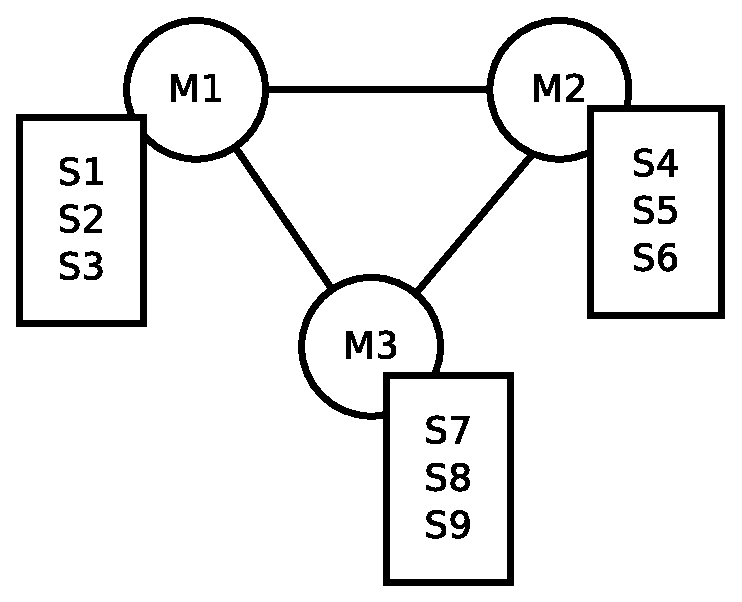
\includegraphics[scale=0.30]{graph2.eps}
  \label{fig:vss:graph2}
\end{figure}

\end{frame}

%----------------------------------

\begin{frame}{Experimental results - Data sets}

\begin{itemize}
\item Movie Reviews\citep{Pang+Lee:04a}

\begin{itemize}
\item 2000 movie reviews: 1000 positive and 1000 negative
\item 100 features
\end{itemize}

\begin{table}[ht]
\centering
\begin{tabular}{ l c }
    \hline\hline
    Algorithm & Accuracy \\ [0.2ex]
    \hline
    Maximum Entropy &  86.33 \\ % 84.92462, 83.91959, 87.9397, 84.92462, 89.94472
    Naive Bayes & 85.62 \\ % 86.43216, 89.447235, 81.407036, 86.43216, 84.42211
    \hline
  \end{tabular}
\label{table:mrprecision}
\end{table}

\end{itemize}

\end{frame}

%----------------------------------

\begin{frame}{Experimental results - Data sets}

\begin{itemize}
\item 20 Newsgroups \footnote{people.csail.mit.edu/jrennie/20Newsgroups}

\begin{itemize}
\item 25000 messages taken from 20 newsgroups
\item 18846 training examples, and 7532 test examples
\item 20 categories: alt.atheism, comp.graphics, comp.os.ms-windows.misc, etc...
\item 5000 features
\end{itemize}

\begin{table}[ht]
\centering
\begin{tabular}{ l c }
    \hline\hline
    Algorithm & Accuracy \\ [0.2ex]
    \hline
    Maximum Entropy &  57.44 \\
    Naive Bayes & 92.12  \\
    \hline
  \end{tabular}
\label{table:20nprecision}
\end{table}

\end{itemize}

\end{frame}

%----------------------------------

\begin{frame}{Experimental results - Data sets}

\begin{itemize}
\item Wikipedia INEX 2009 collection \citep{conf/btw/SchenkelSK07}

\begin{itemize}
\item Prepared for evaluating information retrieval tasks
\item 2,666,190 articles from Wikipedia; we use a subsets of 40,000 articles
\item 331 categories taken from dbpedia\footnote{dbpedia.org/About}: person, song, newspaper, etc...
\item 10000 features
\end{itemize}

\end{itemize}

\end{frame}

%----------------------------------

\begin{frame}{Experimental results - Maximum Entropy Benchmarks}

\begin{itemize}

\item{Vertex for a set of sample}

\begin{itemize}
\item Average improvement of 1.65x times for every 2 cores
\item The biggest improvement is between 1 and 2 cores - 1.86x times
\item The overall improvement between 1 and 8 cores is 7.38x times
\end{itemize}

\begin{figure}[!htb]
  \centering
  \includegraphics[scale=0.35]{maxent_plot.png}
  \label{fig:maxent_plot}
\end{figure}

\end{itemize}

\end{frame}

%----------------------------------

\begin{frame}{Experimental results - Maximum Entropy Benchmarks}

\begin{itemize}

\item{Vertex for every sample}

The average time for this strategy on 8 cores is 5241952 ms which around 111x times worse then the time for vertex for set of samples strategy.

\item{Sequential}

\begin{itemize}
\item No improvement between 1 and 8 cores
\item Parallel version is only 1.40x times then the sequential version
\end{itemize}

\begin{table}[!htb]
\centering
\begin{tabular}{ l c }
    \hline\hline
    Cores & Avarage Time \\ [0.2ex]
    \hline
    1 & 67235 \\
    8 & 67140  \\
    \hline
  \end{tabular}
\label{table:maxentres2}
\end{table}

\end{itemize}

\end{frame}

%----------------------------------

\begin{frame}{Experimental results - Naive Bayes Benchmarks}

\begin{itemize}

\item{Vertex for a set of sample}

\begin{itemize}
\item Average improvement of 1.52x times for every 2 cores
\item The biggest improvement is between 1 and 2 cores - 1.79x times
\item The overall improvement between 1 and 8 cores is 5.25x times
\end{itemize}

\begin{figure}[!htb]
  \centering
  \includegraphics[scale=0.35]{naivebayes_plot.png}
  \label{fig:naive_plot}
\end{figure}

\end{itemize}

\end{frame}

%----------------------------------

\begin{frame}{Experimental results -  Naive Bayes Benchmarks}

\begin{itemize}

\item{Vertex for every sample}

The average time for this strategy on 8 cores is 62300.5 ms which around 38x times worse then the time for vertex for set of samples strategy.

\item{Sequential}

\begin{itemize}
\item No improvement between 1 and 8 cores
\item Parallel version is only 3.10x times then the sequential version
\end{itemize}

\begin{table}[!htb]
\centering
\begin{tabular}{ l c }
    \hline\hline
    Cores & Avarage Time \\ [0.2ex]
    \hline
    1 & 5224.75 \\
    8 & 5579.75  \\
    \hline
  \end{tabular}
\label{table:naivebayes2}
\end{table}

\end{itemize}

\end{frame}

%----------------------------------

\begin{frame}{The end}
Questions ?
\end{frame}

\begin{frame}[allowframebreaks]{References}
\bibliographystyle{plainnat}
\bibliography{references}
\end{frame}

\end{document}